\let\negmedspace\undefined
\let\negthickspace\undefined
\documentclass[journal]{IEEEtran}
\usepackage[a5paper, margin=10mm, onecolumn]{geometry}
%\usepackage{lmodern} % Ensure lmodern is loaded for pdflatex
\usepackage{tfrupee} % Include tfrupee package

\setlength{\headheight}{1cm} % Set the height of the header box
\setlength{\headsep}{0mm}     % Set the distance between the header box and the top of the text

\usepackage{gvv-book}
\usepackage{gvv}
\usepackage{cite}
\usepackage{amsmath,amssymb,amsfonts,amsthm}
\usepackage{algorithmic}
\usepackage{graphicx}
\usepackage{textcomp}
\usepackage{xcolor}
\usepackage{txfonts}
\usepackage{listings}
\usepackage{enumitem}
\usepackage{mathtools}
\usepackage{gensymb}
\usepackage{comment}
\usepackage[breaklinks=true]{hyperref}
\usepackage{tkz-euclide}
\usepackage{listings}                                     
\def\inputGnumericTable{}                                 
\usepackage[utf8]{inputenc}                                
\usepackage{color}                                            
\usepackage{array}                                            
\usepackage{longtable}                                       
\usepackage{calc}                                             
\usepackage{multirow}                                         
\usepackage{hhline}                                           
\usepackage{ifthen}                                           
\usepackage{lscape}
\renewcommand{\thefigure}{\theenumi}
\renewcommand{\thetable}{\theenumi}
\setlength{\intextsep}{10pt} % Space between text and floats

\numberwithin{equation}{enumi}
\numberwithin{figure}{enumi}
\renewcommand{\thetable}{\theenumi}

% Marks the beginning of the document
\begin{document}
\bibliographystyle{IEEEtran}

\title{Question-9.3.11.3}
\author{EE24BTECH11048-NITHIN.K} 
%\maketitle
%\newpage
%\bigskip
{\let\newpage\relax\maketitle}
\textbf{Question:} \\
Solve the differential equation $\frac{d^2y}{dx^2} + 1 = 0$ with initial conditions $y\brak{0} = 1$ and $y^{\prime}\brak{0} = 0$
\textbf{Theoritical Solution:} \\
Laplace Transform :\\
\begin{align}
	\mathcal{L}\brak{f\brak{t}} = \int_{0}^{\infty}e^{-st}f\brak{t}dt
\end{align}
Properties of Laplace tranform
\begin{align}
	\mathcal{L}\brak{y^{\prime\prime}} &= s^2\mathcal{L}\brak{y} -sy\brak{0}-y^\prime\brak{0}
\end{align}
\begin{align}
	\mathcal{L}\brak{1} &= \frac{1}{s}
\end{align}
\begin{align}
	\mathcal{L}^{-1}\brak{\frac{2}{s^3}} &= x^2u\brak{x}
\end{align}
\begin{align}
	\mathcal{L}\brak{cf\brak{t}} &= c\mathcal{L}\brak{f\brak{t}}
\end{align}
Applying the properties to the given equation
\begin{align}
	y^{\prime\prime} + 1 &= 0
\end{align}
\begin{align}
	\mathcal{L}\brak{y^{\prime\prime}} + \mathcal{L}\brak{1} &= 0
\end{align}
\begin{align}
	s^2\mathcal{L}\brak{y} -sy\brak{0}-y^\prime\brak{0}+\frac{1}{s} &= 0
\end{align}
Substituting the initial conditions gives
\begin{align}
	s^3\mathcal{L}\brak{y} + 1 &= 0
\end{align}
\begin{align}
	\mathcal{L}\brak{y} &= \frac{-1}{s^3}
\end{align}
\begin{align}
	y = \mathcal{L}^{-1}\brak{\frac{-1}{s^3}}
\end{align}
\begin{align}
	y = \frac{-1}{2}\mathcal{L}^{-1}\brak{\frac{2}{s^3}}
\end{align}
\begin{align}
	y = \frac{-1}{2}x^2u\brak{x}
\end{align}

\textbf{Computational Solution:} \\
Finite Difference Approximation \\
The second derivative $\frac{d^2y}{dx^2}$is replaced by:\\
\begin{align}
	\frac{d^2y}{dx^2} \approx \frac{y_{n+1} - 2y_n + y_{n-1}}{\Delta x^2}
\end{align}
Substitute this into the differential equation:
\begin{align}
	\frac{y_{n+1} - 2y_n + y_{n-1}}{h^2} + 1 = 0
\end{align}
\begin{align}
	y_{n+1} - 2y_n + y_{n-1} + h^2 = 0
\end{align}
\begin{align}
	y_{n+1} = 2y_n - y_{n-1} - h^2
\end{align}
If $y\brak{0} = 0$, then $y_0 = 0$. \\
To compute $y_1$, use the derivative approximation:
\begin{align}
	y^{\prime}\brak{0} \approx \frac{y_1 - y_0}{h}
\end{align}
\begin{align}
	y_1 = 0
\end{align}



\begin{figure}[H]
    \centering
    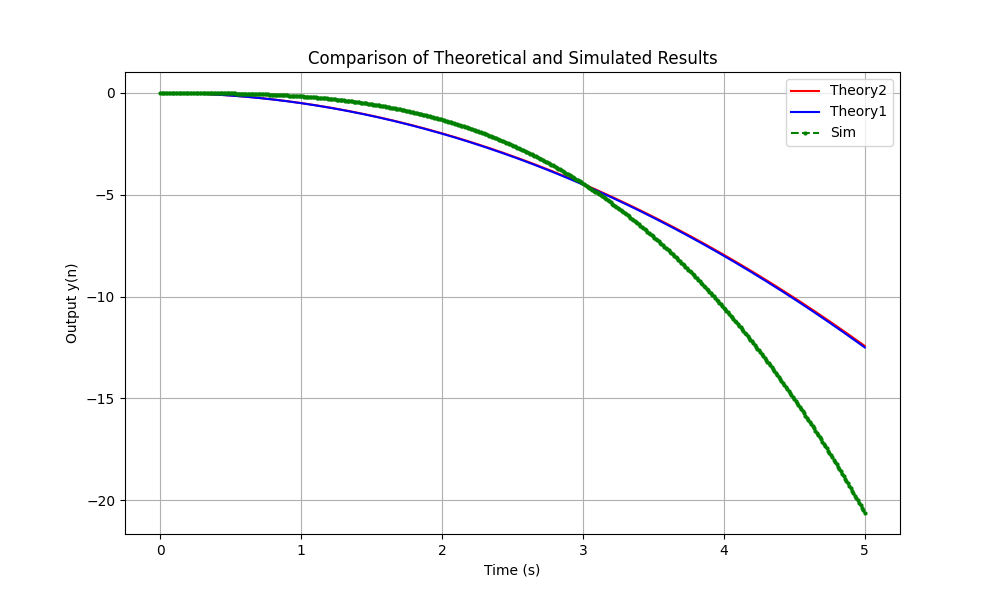
\includegraphics[width=0.8\textwidth]{figs/fig.png}
    \caption{Plot}
\end{figure}


\end{document}
